\documentclass[letterpaper]{article} % DO NOT CHANGE THIS
\usepackage[submission]{aaai2027} % DO NOT CHANGE THIS
\usepackage[hyphens]{url} % DO NOT CHANGE THIS
\usepackage{graphicx} % DO NOT CHANGE THIS
\urlstyle{rm} % DO NOT CHANGE THIS
\def\UrlFont{\rm} % DO NOT CHANGE THIS
\usepackage{natbib} % DO NOT CHANGE THIS
\usepackage{caption} % DO NOT CHANGE THIS
\frenchspacing % DO NOT CHANGE THIS
\nocopyright

\pdfinfo{
/TemplateVersion (2027.1)
/Subject (Anonymous AAAI-27 demonstration paper)
}

\setcounter{secnumdepth}{0}

\title{ContextLens: An Evidence-Grounded Agent for Verifiable Historical Address Investigation}
\author{Anonymous Submission}
\affiliations{}

\begin{document}
\maketitle

\begin{abstract}
Historical addresses are unstable search objects. A place may acquire successive street names, several candidates may remain plausible, and archival coverage is uneven. \emph{ContextLens} compiles an address and era into an inspectable dossier organized around identity, events, spatial context, and sources. A temporal resolver precedes retrieval, while relation and claim gates determine which records may support the reported account. Each record retains a Source Passport containing its provider, dataset, period, identifier, normalization state, and original URI. The demonstration follows a 1934 Shanghai address from query to source record, then examines ambiguous and unresolved inputs.
\end{abstract}

\begin{figure}[t]
  \centering
  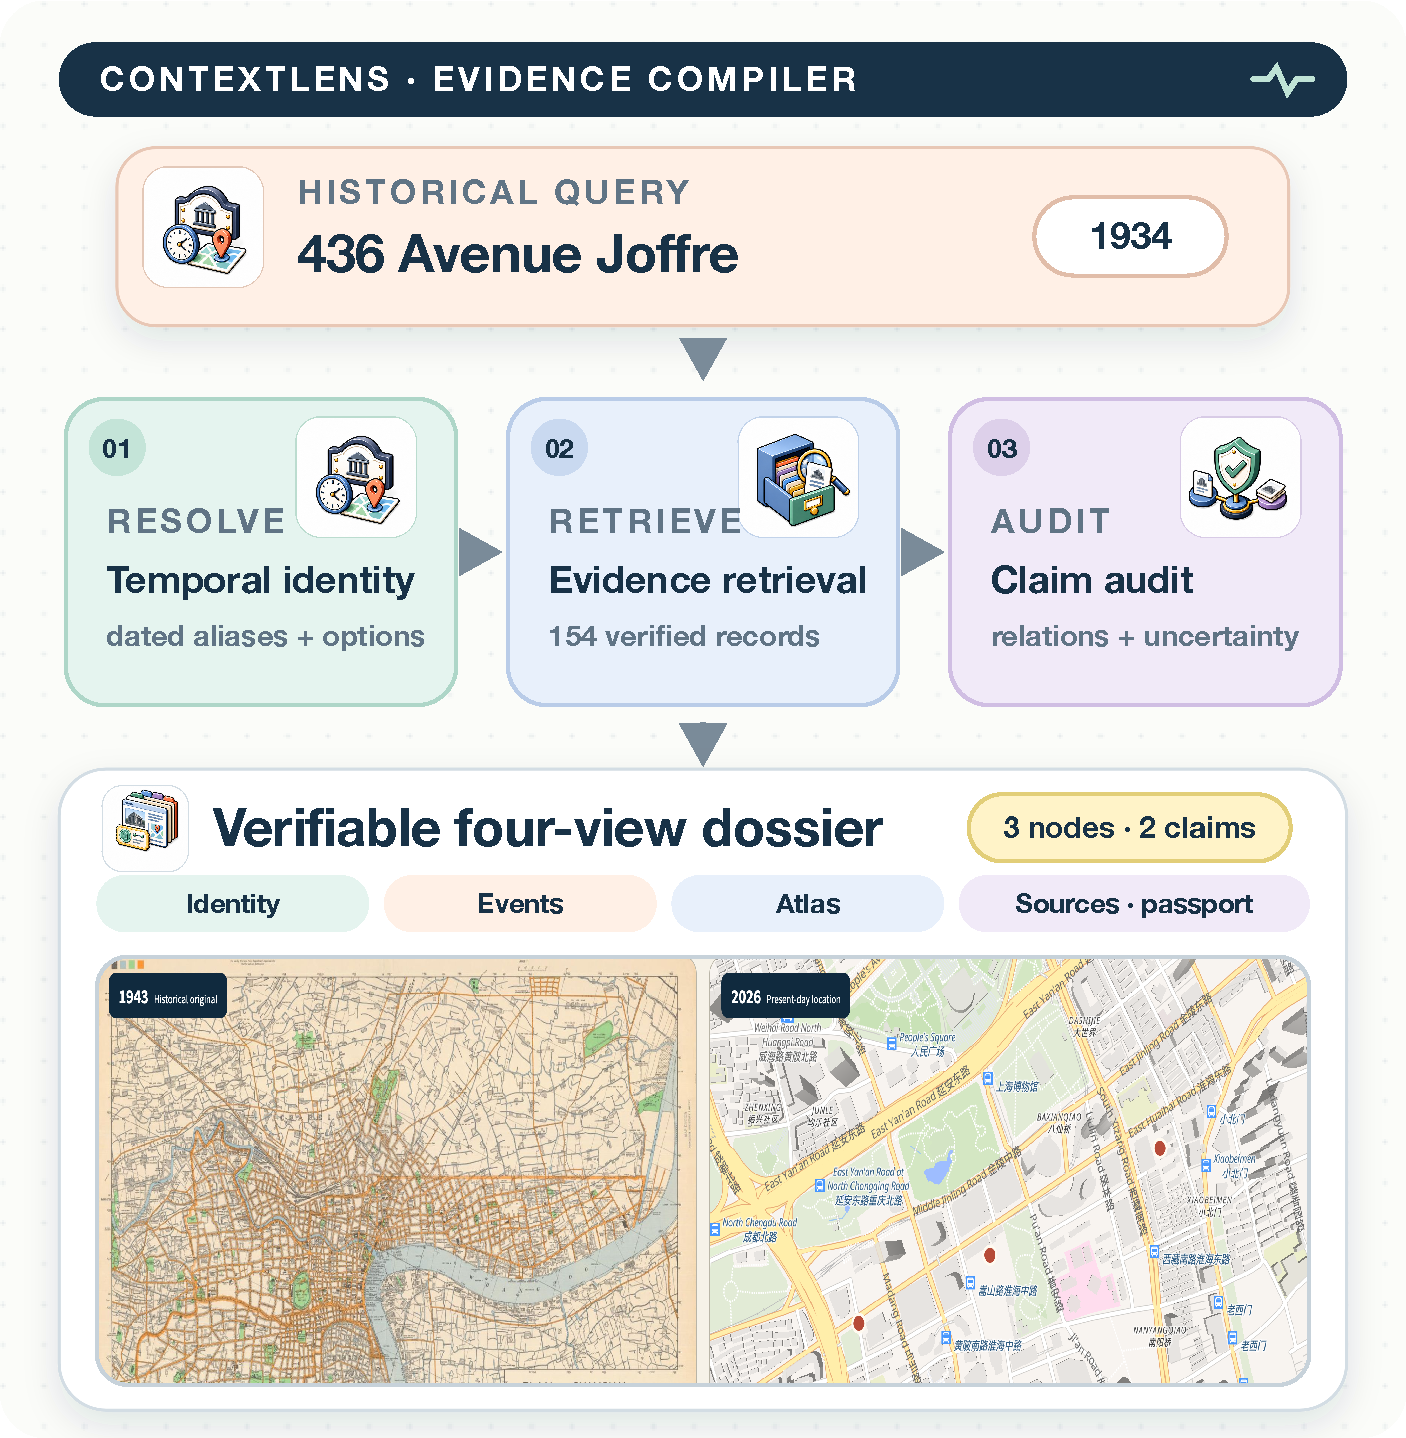
\includegraphics[width=0.815\columnwidth]{assets/contextlens_teaser.pdf}
  \caption{ContextLens resolves a dated place, retrieves evidence, and audits claims before the four-view dossier; the Atlas pairs an archival scan with the modern map.}
  \label{fig:teaser}
\end{figure}

\section{Background and Design Rationale}
Retrieval-augmented generation conditions a response on external collections \cite{lewis2020rag}, and citation-oriented systems expose passages used during generation \cite{gao2023alce}. Neither operation alone determines which historical place a dated street name denotes. Geoparsers ground place mentions in digitized collections \cite{grover2010geoparser}, and toponym-resolution methods rank candidate locations from textual context \cite{delozier2015toponym}. Historical gazetteers further require alternative names, temporal attestations, and explicit uncertainty \cite{southall2011gazetteers}.

Linked-data initiatives connect cultural records through stable place references \cite{isaksen2014pelagios}, while Recogito retains editorial control over semantic and geographic annotation \cite{simon2017recogito}. Semantic portals make heterogeneous cultural data available for interactive investigation \cite{hyvonen2020semanticweb}. ContextLens combines these ideas in a dated-address workflow. It resolves place identity before retrieval and keeps the evidence for each claim inspectable. Competing candidates remain visible when resolution is uncertain.

\section{System Design}
ContextLens represents each query as a place expression, an optional house number, and a temporal constraint. Resolution compares this representation with dated road-name periods and retains candidate identities together with the evidence and rationale for each match. The resulting candidate set constrains downstream retrieval, while the same evidence objects remain available across the dossier shown in Figure~\ref{fig:teaser}.

Resolved candidates guide retrieval over the packaged offline snapshot. It contains 154 verified records across the Shanghai Library's road and place-name, event, building, person, and organization data families \cite{shlibrary2026data}. Normalization preserves the provider, dataset, official URI, evidence identifier, and version used by the interface. Historical scans remain linked to catalog records or image services such as IIIF \cite{iiif2020image}.

Relations between events or entities and places are admitted only when their address, temporal, and source signals are compatible. The claim audit requires a statement to reference an admitted relation and at least one evidence identifier. Records with weaker support remain contextual rather than being phrased as direct claims. The intermediate representation also preserves unresolved candidates, making the boundary between retrieved context and asserted interpretation explicit.

The four coordinated views, \textsc{Identity}, \textsc{Events}, \textsc{Atlas}, and \textsc{Sources}, reference the same evidence objects.

Provenance is represented as interface data rather than a citation string attached after generation. This design follows the distinction between entities, activities, and provenance relations formalized by PROV-O \cite{lebo2013provo}, without claiming full PROV-O conformance. An evidence card and its Source Passport share an identifier, and claim links use that identifier to reopen the supporting record. The source table separates the collection total from the evidence returned for the current address. A dossier-level JSON representation preserves the same claim links.

An optional language model can summarize admitted evidence after relation auditing. Its prompt contains evidence cards, typed relations, and identity-audit states, and requires historical statements to cite supplied identifiers. Returned identifiers are intersected with the admitted set, which discards unsupported references while preserving stated uncertainties. This division assigns linguistic synthesis to the model while resolution, relation admission, and provenance validation remain explicit system operations. If generation is disabled or fails, the evidence dossier remains available unchanged.

\section{Demonstration Scenario}
% Anonymous artifact repository (for the authors; omit web pointers from the review PDF):
% https://anonymous.4open.science/r/ContextLens-B7C0/README.md
The demonstration centers on ``436 Avenue Joffre, 1934.''\footnote{The complete source code and demonstration video are provided in the supplementary materials.} The resolver associates Avenue Joffre with the present-day Huaihai Middle Road area and reconstructs six dated road names. The resulting dossier contains three spatiotemporal nodes and two direct claims. One admitted claim connects the 1934 founding of Kangjian Bookstore to No.~436. The statement remains bounded by the supporting event record and its temporal scope.

Dated names, timeline events, and map context are projections over a shared evidence layer. Claim links and timeline entries reference the same evidence objects as the \textsc{Sources} view. In the main case, the 1934 event, its Source Passport, and the original URI remain connected by a single evidence identifier.

\textsc{Identity} displays dated names, while \textsc{Events} orders the admitted records. \textsc{Atlas} places a 1943 scan beside the modern map and states that the scan is unsuitable for precise house-number alignment. \textsc{Sources} lists four evidence cards with openable official records. Three distinct source records support the direct claims reported in the dossier. The Source Passport associated with each card retains its provenance fields and original URI, as illustrated in Figure~\ref{fig:sources}.

Ambiguous and unresolved inputs remain part of the same interaction. ``Nanjing Road department store'' retains multiple road candidates for review. A synthetic address absent from the snapshot is assigned an unresolved state with a request for additional evidence. These paths use the packaged evidence and remain available without network access. All 29 functions in the local Python test suite pass, covering address lineage, ambiguity, negative cases, relation gating, network failure, privacy logging, and interface contracts. This check concerns implementation behavior; no retrieval accuracy or user-study result is claimed.

\begin{figure}[t]
  \centering
  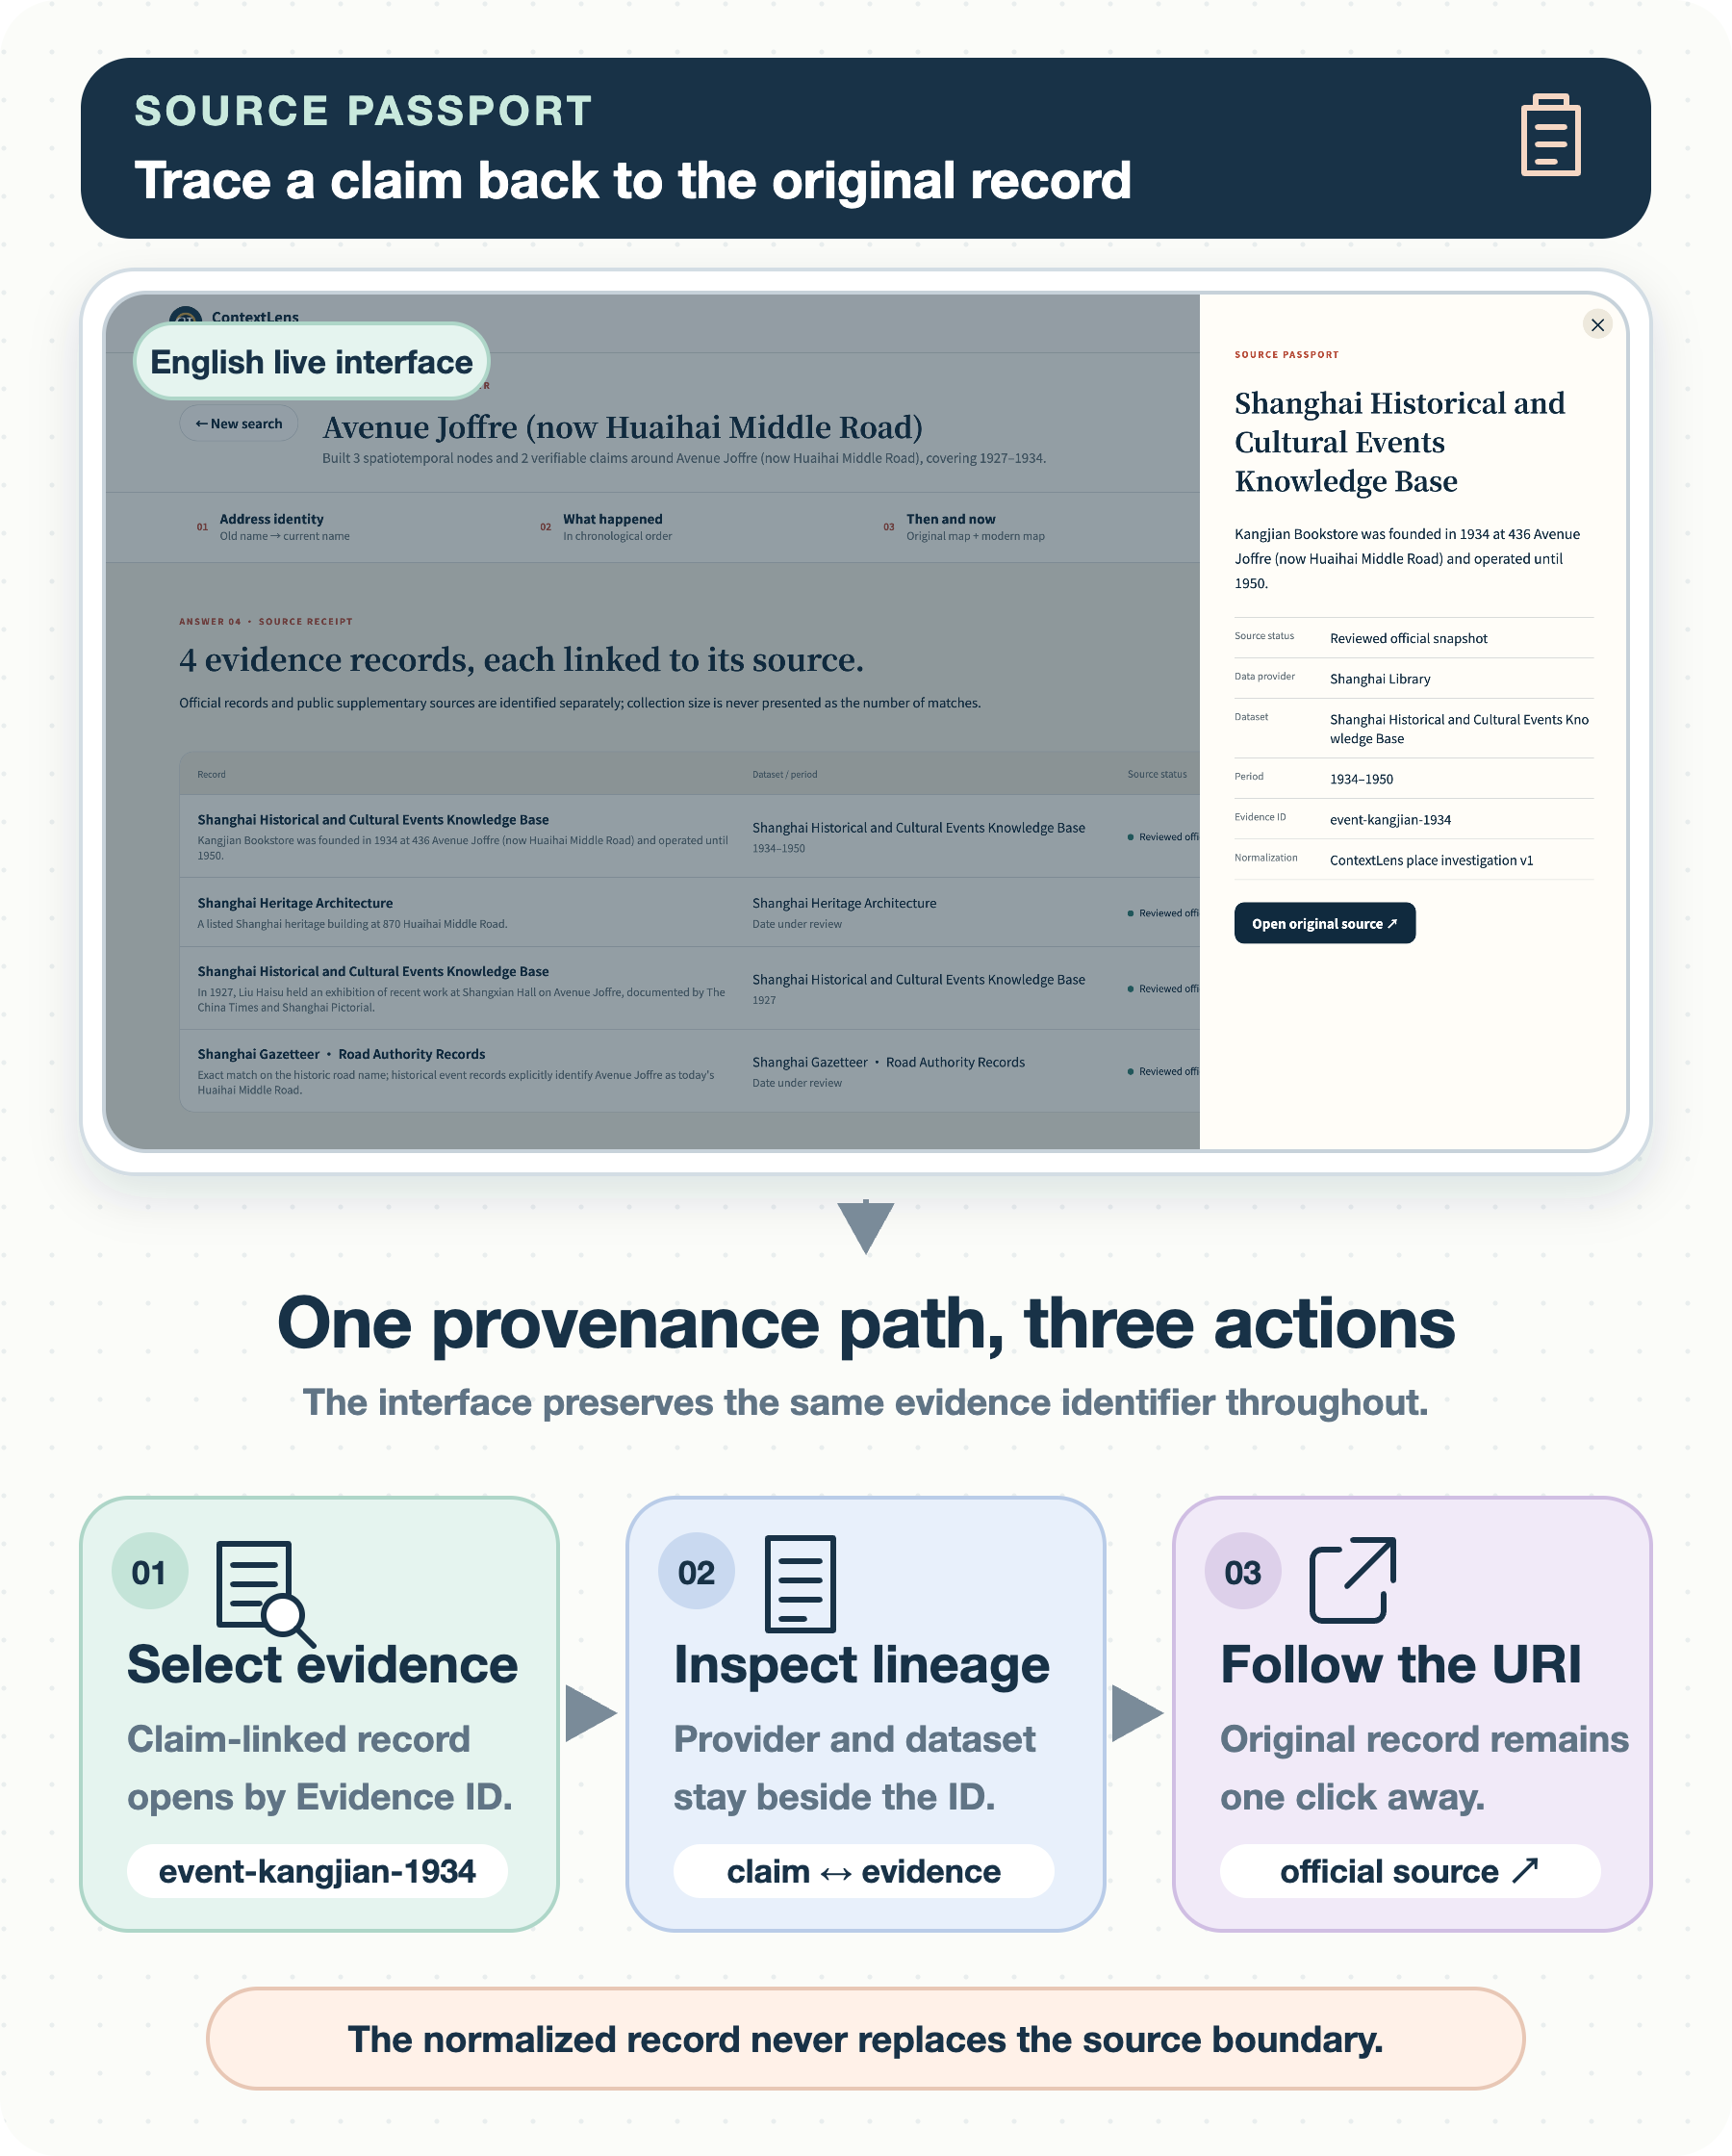
\includegraphics[width=0.96\columnwidth]{assets/contextlens_sources_figure.png}
  \caption{The English Sources view shows how an evidence identifier connects a claim to provenance fields and the original URI.}
  \label{fig:sources}
\end{figure}

%\section{Design Boundaries and Scope}
%The interface withholds a claim when no supporting record is available and preserves ambiguity in the resolver output. Its archival map supports visual orientation but is not treated as a registered house-number layer. Official records and auxiliary public maps are labeled separately so that their evidential roles are not conflated.

%The current snapshot is Shanghai-specific and small relative to the underlying collections. Name-period rules require maintenance, and some coordinates are coarse. ContextLens is therefore an investigation interface rather than a general historical geocoder. The system has not yet been evaluated with historians or public users. Language-model assistance is optional. Identifier gating prevents unsupported provenance links but cannot establish the historical adequacy of the underlying records. Evaluation of resolution quality and expert correction workflows remains future work.

\section{Design Boundaries and Scope}
The interface withholds a claim when no supporting record is available and preserves ambiguity in the resolver output. Its archival map supports visual orientation but is not treated as a registered house-number layer. Official records and auxiliary public maps are labeled separately so that their evidential roles are not conflated. Source Passports establish provenance but do not guarantee the historical completeness or correctness of the underlying records.

The current snapshot is Shanghai-specific and small relative to the underlying collections. Name-period rules require maintenance, some coordinates are coarse, and archival gaps may leave valid addresses unresolved. ContextLens is therefore an investigation interface rather than a general geocoder. Identifier gating prevents unsupported provenance links but cannot establish the historical adequacy of evidence. The system has not yet been evaluated with historians or public users. Evaluation of resolution accuracy, broader coverage, and expert correction workflows remains future work.

\section{Conclusion}
ContextLens connects temporal place resolution to evidence inspection within a single historical-address workflow. Model-assisted interpretation remains secondary to the claim and provenance structures that support the dossier. Ambiguous and unresolved inputs are preserved for review rather than converted into confident historical claims.



\clearpage
\bibliography{contextlens_references}
\end{document}
